\documentclass[conference]{IEEEtran}
\IEEEoverridecommandlockouts
\usepackage{graphicx}
\usepackage{algorithm}
\usepackage{algorithmicx}
\usepackage{algpseudocode}
\usepackage[dvipsnames]{xcolor}
\usepackage{amsmath}
\usepackage{hyperref}

\algblock{Input}{EndInput}
\algnotext{EndInput}
\algblock{Output}{EndOutput}
\algnotext{EndOutput}
\newcommand{\Desc}[2]{\State \makebox[2em][l]{#1}#2}

\newcommand{\tristan}[1]{\color{orange}\textbf{From Tristan:}#1\color{black}}


\begin{document}
\title{I/O simulation model with Linux page cache, integration and evaluation in SimGrid framework}

\author{\IEEEauthorblockN{Hoang-Dung Do, Val\'erie Hayot-Sasson, Tristan Glatard
  }\\
  \IEEEauthorblockA{
    Department of Computer Science and Software Engineering, Concordia University, Montreal, Canada
  }
}

\maketitle

	\begin{abstract}
		\begin{itemize}
			\item The I/O bottleneck in HPC and the need of experiments.
			\item HPC experiment frameworks and advantages of SimGrid.
			\item The missing of the ability to simulate page cache, the goal of this paper.
			\item Principle of the simulator, experiment scenarios and comparisons.
			\item Brief discussion on results and future work.
		\end{itemize}
	\end{abstract}

	\section{Introduction}
		\begin{itemize}
			\item HPC, the bottleneck in I/O and the demand of HPC experiments. 
			\item Difficulties in conducting high performance computing experiments and the need of simulation frameworks.
			\item Existing experiment methods, simulators, simulation frameworks. The advantages of SimGrid compared to others \cite{casanova2008, lebre2015}. The missing of the ability to simulate page cache in SimGrid \cite{lebre2015}.
			\item The objective of the paper: Add capability to simulate I/O with page cache in SimGrid.
		\end{itemize}
	\section{Related Work}			
		
		\subsection{Page cache}
			\begin{itemize}
				\item What is page cache? How it works \cite{linuxdev3rd2010}. Effects and importance of page cache.
				\item Introduce some existing strategies with some highlighted pros and cons.
				\item Current implementation in Linux and some reasons why it is chosen to be implemented (implementation complexity, effectiveness, overhead, etc) \cite{linuxdev3rd2010}
				\item \tristan{LRU lists are mentioned in the next section, they should be described here.}
			\end{itemize}									

		\subsection{Simulators}
			\begin{itemize}
				\item Discuss some existing methods, simulation frameworks to conduct HPC experiments. Compare pros and cons (accuracy, simulation time, usability) of some simulators (SimGrid, GridSim).
				\item Related development: RAM energy consumption \cite{gill2019} \cite{ouarnoughi2017} 
				\item Discuss the pros of SimGrid and the reasons why we chose it to extend. (Section 2.2.2 in \cite{casanova2014})
				\item \tristan{Mention the status of storage simulation in simulators, so that we understand from Fig 1 that storage devices are available}
			\end{itemize}
			
	\section{Method}
		In this section, we present our approach to model file read/write,
		memory I/O, cache eviction and data flushing mechanisms implemented in
		the Linux kernel. We also detail the design of our simulators and their
		implementation. Finally, we describe experimental scenarios to evaluate
		our simulation model on real applications using a standalone Python
		prototype, the current SimGrid simulator, and our extension of SimGrid.

		\subsection{Principle of the simulator}
	
            We separate our simulation model in two components, the IO
			Controller and the Memory Manager, which together simulate Linux
			kernel I/Os (Figure~\ref{fig:interaction}). The Memory Manager
			simulates memory I/O, flushing, and cache eviction, whereas the IO
			Controller simulates file reads and writes. Simulated applications
			can simply interact with the IO Manager instead of calling simulated
			storage directly as is the case with current simulators.

			\begin{figure}
   				\centering
   				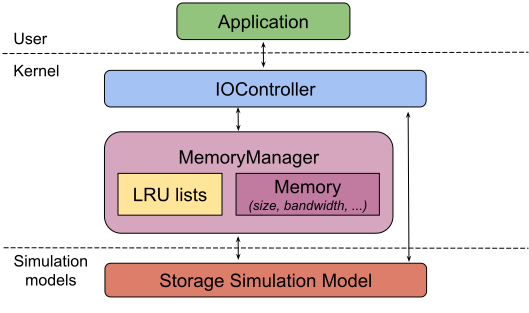
\includegraphics[width=0.85\columnwidth]{figures/interaction.pdf}
   				\caption{Overview of the simulated write-back page cache}\label{fig:interaction}
			\end{figure}	

			\subsubsection{Memory simulation model}
			
			We model memory as a storage device, characterized with a capacity,
			a read bandwidth and a write bandwidth in most simulators
			\tristan{are the read and write bandwidths distinguished in simgrid?
			we should also talk about latency}. We refer to existing simulation
			models for storage devices, to simulate bandwidth sharing for
			parallel accesses \tristan{we should refer to related work, see
			comment there}.

			We introduce the concept of a data block as a unit to represent data
			cached in memory. A data block is a subset of file pages stored in
			page cache that were accessed in the same read or write
			operation. A data block
			has information about file name, block size, last access time, and a
			dirty flag that represents whether the data is clean (0) or dirty
			(1). A given file can have multiple data blocks in page cache. In
			addition, a data block can be split into an arbitrary number of
			smaller blocks, and data blocks can be merged together.
			\tristan{I reformulated this paragraph, please check}
			
			We simulate the kernel LRU lists of file pages
			with two lists of data blocks: an active list and 
			an inactive list, ordered by last access time (earliest first, see Figure~\ref{fig:lrulist}).
			As in the kernel, our simulator keeps the size of the active list under
			twice the size of the inactive list by moving least recently 
			used data blocks from the active list to the inactive list. 
			Modeling page cache LRU lists as lists of data blocks reduces the
			overhead of the simulator, as data blocks are obviously less
			numerous than file pages, while preserving the accuracy in I/O time
			simulation \tristan{how do you know that, can you provide an argument?}.

			\begin{figure}
   				\centering
   				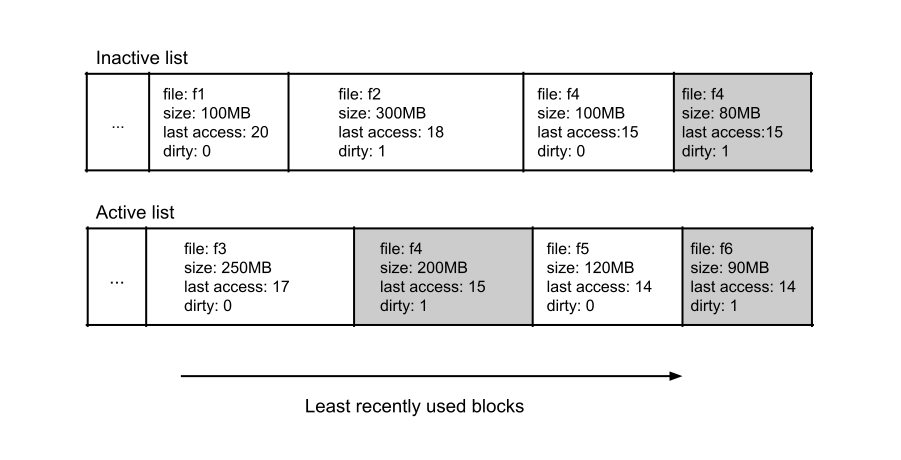
\includegraphics[width=\columnwidth]{figures/lru_lists.pdf}
   				\caption{Simulation of page cache LRU lists with data blocks}\label{fig:lrulist}
			\end{figure}	
			
			
			\tristan{is this paragraph about read accesses or write accesses? I
			think you should make one for reads, and one for writes. The
			paragraph could start as follows: ``The simulated LRU lists are used
			as follows. When a file is accessed, \ldots ''} At the time when a
			file is accessed, some data of the file can be in cache or not. If
			accessed data is already cached, there are existing data blocks
			representing cached data in two page cache LRU lists. 
			As cached data is accessed again, these blocks are moved to 
			the active list, dirty blocks are merged into a bigger dirty block, 
			while clean data blocks are merged into another clean block. 
			If accessed data is not in cache, new blocks representing uncached data 
			are created and put into the top of the inactive list. 
			For more detail when uncached data is accessed, in the case of 
			reading file, as all uncached data is clean data, only one clean data 
			block is added to the inactive list.
			But in the case of writing uncached file data though cache, 
			this written data can be either dirty or clean. 
			Thus, at most two data blocks can be added to the inactive lists, 
			one is clean and one is dirty. 
			We also keep the size of the active list not larger than twice the size of 
			the inactive list as in the kernel. This is done by moving least recently 
			used blocks in the active list to the inactive list when the active list 
			grows. If only a part of a data block needs to be moved, 
			the block is split.

			Next, we simulate data flushing mechanism, which writes back 
			dirty data to disk. 
			The data flushing simulation function traverses the sorted inactive first, 
			and then the active list, looks for least recently used dirty blocks \tristan{, writes them to disk through the storage device model,} and 
			sets dirty flags of these blocks to 0 until the total flushed amount 
			reaches the amount to be flushed or there is no dirty data left in cache. 
			If the last flushed block is not entirely flushed, it is split into 
			two blocks, one that is flushed and one that remains dirty.
			The flushing time is simulated with storage model.
			
			For periodical flushing, our simulator searches in two page cache 
			LRU lists and flushes all the expired dirty data blocks. 
			A dirty data block is considered expired if the time from its last access 
			to current simulated time is longer than the predefined expire time. 
			Periodical flushing can be concurrent with cache read/write, 
			and sequential with disk read/write. When cache accesses and 
			periodical flushing are concurrent, flushing time is not added to simulated 
			time but the amount of flushed data is limited by flushing time. 
			When data is flushed in parallel with disk read/write, flushing time is 
			calculated by storage simulation model and total amount of data 
			to be flushed \tristan{This concurrency should be handled by the storage model, not the memory manager described here. 
			Rephrase the last sentences to explain this.}.
				
			Similarly to data flushing, our cache eviction simulation function frees up 
			the page cache by traversing and deleting least recently used clean 
			data blocks in the inactive list.
			The amount of evicted data is passed in and data blocks are deleted 
			from the inactive list until total evicted data reaches the amount 
			passed in, or there is no clean block left in the list.
			If the last evicted block is not entirely evicted, the block is split, 
			and only one block is deleted.
			Our cache eviction simulation does not add up to the simulated time 
			since cache eviction time is negligible in real systems.			
			
            \tristan{very good writing Dzung, it reads very well now.}

			\subsubsection{File I/O simulation model}			
			
			Simulated applications can simply request for a file read 
			or a file write by calling the IO Controller instead of 
			the storage simulation models. 
			\tristan{this should move, not sure where for now: Because every computer has its own memory and system configurations, 
			one IO Controller object and one Memory Manager object are created 
			for each simulated machine.}
			
			To read or write a file, a simulated application sends a request to the 
			IO Controller instance on the node where the requested file is stored.
			Based on the memory status in Memory Manager, the IOController 
			orchestrates cache reads and writes, disk reads and writes, flushing, cache eviction 
			 and returns to the simulated application.
			
			\begin{algorithm}\caption{File read simulation}\label{alg:read}
				\small
				\begin{algorithmic}[1]
					\Input
        				\Desc{fn}{file name}
        				\Desc{fs}{file size (assumed to fit in memory)}
						\Desc{rt}{current simulated run time}
						\Desc{mm}{MemoryManager object}
						\Desc{rm}{memory read bandwidth}
						\Desc{sm}{storage simulation model}
   					\EndInput
   					\Output
						\Desc{rt}{simulated run time after the file is read}
   					\EndOutput
					\State rt = rt + mm.flush(2*fs - mm.cached(fn) - mm.evictable\_mem) 
					\State mm.evict(2*fs - mm.cached(fn) - mm.free\_mem) 
					\If {mm.cached(fn) $>$ 0}  \Comment{Read file cached data}
    					\State crt = mm.cache\_read(fn)  \Comment{Read data in cache}
    					\State mm.periodic\_flush(rt, crt) \Comment{Flush in duration = crt}
						\State rt = rt + crt
					\EndIf
					\If {mm.cached(fn) $<$ fs} \Comment{Read uncached data from disk}
						\State rt = rt + mm.periodic\_flush(rt) \Comment{Sequential flushing}
						\State mm.disk\_read(fs - mm.cached(fn), fn)
    					\State rt = rt + sm.read(fs - mm.cached(fn))
					\EndIf					
					
					\State \Return rt
					
				\end{algorithmic}
			\end{algorithm}			
			
			The algorithm to simulate file reads is described in 
			Algorithm~\ref{alg:read} \tristan{you should now remove the incrementation of simulation time, as the storage models will do that.
			Essentially, we neglect kernel time and assume that time is entirely spent in IO. It will simplify the algorithms further, which is also elegant. If you 
			agree, please revise the algorithm and its description accordingly, and do the same for algorithm 2.
			}.  
			In Linux systems with write-back storage devices, data can be either read 
			from cache with memory bandwidth or read from disk with disk bandwidth. 
			Therefore, total read time can be considered as a linear function 
			of the read time with each of these bandwidths, 
			enabling us to generalize reading process as two separate phases, 
			cache read and disk read. 
			When a simulated application reads a file, 
			it sends a file read request to IO Controller. 
			First, if there  is not enough memory available to store two
			copies of the file (one in cache, one in anonymous memory), the
			Memory Manager is called to flush dirty data to disk (line 10).
			This flushing is complemented by eviction by the Memory Manager (line 11). 
			Next, if the file is cached, either partially or entirely, the Memory Manager is 
			called to read and update the corresponding data blocks in cache (line 13). 
			During cache read, periodical flushing is called to flush dirty data if needed 
			and limited to cache read time \tristan{unclear, reword} (line 14).
			Cache read time is then added to total simulated time (line 15) \tristan{this should be part of the storage model}. 
			If file is not cached or partially cached, a disk read is required (line 17). 
			Periodical flushing is called once again, but not time-limited since 
			data flushing and disk read are sequential, and the flushing time is 
			added to simulated time (line 18).
			Finally, data is read from disk to cache and managed by MemoryManager, 
			disk read time estimated by the storage model is added to 
			total simulated run time (line 19-20). 

			\begin{algorithm}\caption{File write simulation}\label{alg:write}
				\small
				\begin{algorithmic}[1]
					\Input
        				\Desc{fn}{file name}
        				\Desc{fs}{file size}
						\Desc{rt}{current simulated run time}
						\Desc{mm}{MemoryManager object}
						\Desc{wm}{memory write bandwidth}
						\Desc{sm}{storage simulation model}
   					\EndInput
   					\Output
						\Desc{rt}{simulated run time after the file is read}
   					\EndOutput
   					\State pft = mm.periodic\_flush(rt)
					\State remain\_dirty = dirty\_ratio * mm.avail\_mem - mm.dirty
					\State mem\_amt = min(fs, remain\_dirty)
					\If {remain\_dirty $>$ 0} \Comment{Write with memory bandwidth}
    					\State mm.evict(mem\_amt - mm.free\_mem)
    					\State mm.periodic\_flush(rt, mm.write\_time(mem\_amt)) 
    					\State rt = rt + mm.write(fn, mem\_amt)
    				\EndIf
    				\State rt = rt + max(mem\_amt / wm, pft) \Comment{Concurrent processes}
					\If {mem\_amt $<$ fs}  \Comment{Write with disk bandwidth}
						\State mm.flushed(fs - mem\_amt)  \Comment{Concurrent flushing}
						\State mm.evict(fs - mem\_amt  - mm.free\_mem) 
						\State mm.write(fn, min(fs - mem\_amt, mm.free\_mem))
						\State rt = rt + sm.write(fs - mem\_amt)
					\EndIf
					
					\Return rt
					
				\end{algorithmic}
			\end{algorithm}

			Algorithm~\ref{alg:write} describes our simulation of file write. 
			Initially, periodical flushing is called to flush expired dirty data 
			at the beginning of the write (line 10).
			Similar to the file read simulation, a file can also be written with 
			two different bandwidths, memory bandwidth and disk bandwidth. 
			Files can be written with memory bandwidth before the amount 
			of dirty data reaches dirty\_ratio. Thus, our algorithm initially checks 
			the amount of file data that can be written with memory write 
			bandwidth (line 11-12).
			If this amount is greater than 0, MemoryManager is asked to evict 
			data from cache if needed (line 14).
			Next, periodical flushing flushes data during cache write because they 
			can be concurrent (line 15). Then, data is written to cache with memory 
			bandwidth, write time is simulated and added to total simulated 
			time (line 16).
			The amount of data that is not written with memory bandwidth is written 
			with disk bandwidth (line 18). 
			Now, the dirty ratio threshold is reached, we have to flush and evict 
			data from cache as much as possible so that 
			the remaining data can be written to cache (line 20-21). 
			Here, MemoryManager does not guarantee that the amount of flushed 
			and evicted data is enough for the remaining data. In the case it is 
			less than the required amount, the remaining data is written to cache 
			but then can be flushed and evicted right away. Thus, the amount 
			of remaining data that is written and kept in cache after the write 
			is limited by the amount free memory (line 22). 
			Finally, the write time is simulated, added to the total time and 
			returned to simulated applications (line 23).
			
		\subsection{Implementation}

			To validate our simulation model, we create a simple prototype
			simulator independently of existing simulation frameworks and libraries. 
			This enables us to evaluate the accuracy and correctness of our 
			model in a simple scenario before integrating it in the more complex SimGrid environment. 
			In this prototype we use the following basic storage model, used for both memory and disk: 
			\begin{align*}
				& t_{mr} = D / r_m \\ 
				& t_{mw} = D / w_m\
			\end{align*}		
			
			where:
			\begin{itemize}
				\item $t_{mr}$ is the time to read data from memory
				\item $t_{mw}$ is the time to write data to memory
				\item $D$ is the amount of data to read/write
				\item $r_m$ is the memory read bandwidth
				\item $w_m$ is the  memory write bandwidth
			\end{itemize}			
			\tristan{if this applies equally to memory and disk, use ``device'' instead of ``memory''}

			Since bandwidth sharing is not simulated, this prototype doesn't support concurrency: it is limited 
			to single-threaded pipelines running on systems 
			with a single-core CPU. \tristan{the following aren't resulting from the lack of bandwidth sharing simulation, these are more general limitations, I think we 
			should remove them: , a single local storage device, and all input and 
			output files are stored locally.} We use it in a first validation of our simulation model,
			against a real sequential pipeline running on
			a real system.
			
			Having our model validated, we create simulators for different use cases 
			using the current version of SimGrid and the SimGrid version that is 
			extended with our model. To simulate our pipelines and system, we leverage the Workflow Management System Simulation Workbench (WRENCH~\cite{wrench}), a framework  
			built over SimGrid.
		    We compare the results of the simulators with
			original SimGrid and extended SimGrid with the results of real
			pipelines on a real system \tristan{this will have to be updated with a description of extended SimGrid, 
			you should add a placeholder for this description.}. 
		
			We use Python 3.7 to implement the simple simulator, SimGrid 3.25
			and Wrench 1.6 for SimGrid simulators. SimGrid source code is
			available at \url{https://framagit.org/simgrid/simgrid}, and WRENCH
			is at \url{https://github.com/wrench-project/wrench}.
			\tristan{You should also add the URL of your Python prototype}
			
		\subsection{Experiments}
		
			The goal of our experiments is to evaluate our write-back cache
			simulation in single-threaded and multi-threaded applications
			accessing data on different types of file system. We use a pipeline
			of sequential tasks where each task reads an input file, increments
			every byte of the input to emulate real processing and avoid caching
			effects, and writes the result to disk. The output of the previous
			task is the input of the next task. We also use a real application pipeline, to evaluate the applicability of our
			simulation model \tristan{add a placeholder to describe the real pipeline here}.
			
			The simplest execution scenario is single-threaded, where memory 
			bandwidth and disk bandwidth are dedicated. 
			This allows us to compare the detailed results in terms of read/write time, 
			memory states after every single task and, more importantly, validate our 
			simulation model \tristan{last sentence is convoluted, reword}. 
			
			For multi-threaded applications, we vary the number of concurrent
			pipelines running on a multi-core host and writing to the same local
			disk. In this way, we evaluate our model with concurrent I/Os, when
			the device bandwidth is shared.
			
		    Since different storage types should also be taken into account, 
		    we conduct the next experiment with the same scenario as 
		    in the multi-threaded experiment, except that files are stored on a 
		    shared file system instead of local disk. 
		    
		    Finally, we consider a real pipeline from the neuroimaging domain. 
		    We simulate the pipeline with a simulated workflow in SimGrid 
			and compare the simulation results with the real results. 
			Because our work focuses on I/O time, we assume that CPU time is 
			correctly modeled and use the CPU time measured in the real pipelines 
			to setup our simulated workflow \tristan{the pipeline should be described, including the workflow engine if it's Dask.}. 
			
			We use our dedicated cluster hosted at Concordia University to conduct the experiments. The cluster 
			consists of one login node, 8 compute nodes 
			and 4 storage nodes connected with two network switches. The login node 
			has one Intel(R) Xeon(R) Gold 6130 CPU @ 2.10GHz, 128GiB of RAM, 1.8TB 
			of storage of XFS file system, 13GB of tmpfs file system and 385 TB of 
			Lustre shared file system. Each compute node has two 16 cores Intel(R) 
			Xeon(R) Gold 6130 CPU @ 2.10GHz, 256 GB of RAM and 6 SSDs, 450GB each 
			with XFS file system, 378GB of tmpfs and 126GB of devtmpfs file system.
			Lustre file system is configured with one metadata target with 854GB 
			of storage, 44 object storage targets with 8.7TB of storage each. 
			The cluster is run on CentOS 8.1 with the Slurm Workload Manager installed. We use 
			\textbf{\textit{atop}} and \textbf{\textit{collectl}} as tools to monitor 
			and collect data of memory, page cache status and disk throughput on 
			the cluster. The cluster nodes are connected with ... 
			\textcolor{red}{[network description here]}
			\tristan{mention the number of disks on all nodes. Maybe add a diagram.}
	

			\tristan{I don't think you need an intro paragraph for each experiment, as you did above, AND then subsections. I'd just make a single paragraph or sub-section.}
			\subsubsection{Single-threaded evaluation}

				In this experiment, our goal is to validate our model by comparing 
				the simulation results of the simple Python simulator with results of 
				a simulator implemented with original SimGrid, a simulator 
				implemented with SimGrid integrated with our model, and a real pipeline 
				running of the cluster. 
				The pipeline consists of three tasks, each task reads a file, 
				increases every byte and writes output file to local disk. 
				We use the input sizes of 20 GB, 50 GB, 75 GB and 100 GB, run 
				the pipeline on the cluster, measure the CPU time of the pipeline 
				with each input to simulate the pipeline with the simulators.

			\subsubsection{Multi-threaded evaluation}

				In the second experiment, we evaluate the simulator in concurrent I/O 
				with a multi-threaded application. As we run the pipelines on 
				only one compute node of the cluster, which has upto 32 cores per node,  
				we create 32 input files with the size of 3GB each and vary the number of 
				concurrent pipelines from 1 to 32. 
				Because multi-threaded simulator implementation in Python is 
				expensive, and we have our model integrated in SimGrid, 
				we only compare the results of simulators with original SimGrid, 
				SimGrid integrated with our model and and real pipelines. 
				The results are compared in total makespan of the pipelines, 
				cumulative read time and cumulative write time.
			
			\subsubsection{Evaluation on storage types}

				

			\subsubsection{Simulation of a real application}
				A real pipeline (for example a pipeline with nighres)

	\section{Results}
	
		\begin{itemize}

			\item Quantitative results: 
				\begin{itemize}
					\item Errors of simulation time and memory used compared to real results.
					\item Simulation time compared to baseline SimGrid.
				\end{itemize} 

			\item Ability of the model to generalize memory trends (dirty data, cache used) and disk throughput.

		\end{itemize}

	\section{Discussion and Future Work}
		\begin{itemize}
			\item Sensitivity of the simulator on the variation of memory and disk bandwidth. 
		\end{itemize}
	\section{CFI for cluster}
\bibliographystyle{plain}
\bibliography{citation}

\end{document}